\documentclass[11pt]{beamer}
\usepackage[utf8]{inputenc}
\usepackage[english]{babel}
\usepackage{amsmath}
\usepackage{amsfonts}
\usepackage{amssymb}
\usepackage{graphicx}
\usepackage{longtable}
\usepackage{booktabs}
\usepackage[retainorgcmds]{IEEEtrantools}
\usepackage{subcaption}
\usetheme{AnnArbor}
\usecolortheme{beaver}
\begin{document}
\author{Marcelo Ruas e Alexandre Street}
\title{Scenario generation for nongaussian time series via Quantile Regression}
%\subtitle{}
	%\logo{}
	%\institute{}
	%\date{}
	%\subject{}
	%\setbeamercovered{transparent}
	%\setbeamertemplate{navigation symbols}{}
\begin{frame}[plain]
\maketitle
\end{frame}






\section{Introduction}\label{introduction}

\begin{frame}{Motivation}

\begin{itemize}
	\item
	Renewable energy scenarios are important in many fields in Power
	Systems:
	
	\begin{enumerate}
		\def\labelenumi{\roman{enumi})}
		
		\item
		Energy trading;
		\item
		unit commitment;
		\item
		grid expansion planning;
		\item
		investment decisions
	\end{enumerate}
	\item
	In stochastic optimization problems, a set of scenarios is a needed
	input.
	\item
	Robust optimization requires bounds for probable values.
\end{itemize}

\textbf{Change in paradigm: from predicting the conditional mean to
	predicting the conditional distribution}

\end{frame}

\begin{frame}{Probability Forecasting Approaches}

\begin{itemize}

\item
\emph{Parametric Models}

\begin{itemize}
	
	\item
	Assume a distributional shape
	\item
	Low computational costs
	\item
	Faster convergence
	\item
	\emph{Examples: Arima-GARCH, GAS}
\end{itemize}
\item
\emph{Nonparametric Models}

\begin{itemize}
	
	\item
	Don't require a distribution to be specified
	\item
	High computational cost
	\item
	Needs more data to produce a good approximation
	\item
	\emph{Examples: Quantile Regression (Koenker and Bassett Jr (1978)),
		Kernel Density Estimation (Gallego-Castillo et al. (2016)),
		Artificial Intelligence (Wan et al. (2017))}
\end{itemize}
\end{itemize}

\end{frame}

\begin{frame}{Wind Power Time Series - Icaraizinho monthly data}

\begin{figure}
\centering
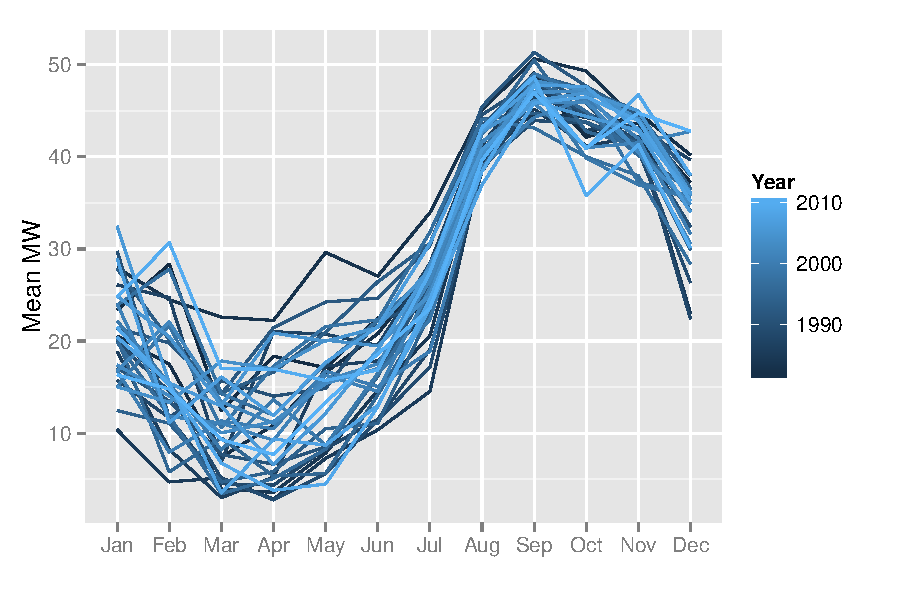
\includegraphics[width=0.9\linewidth]{Images/icaraizinho-mensal}
\end{figure}

\end{frame}

\begin{frame}{Wind Power Time Series - Kaggle forecasting competition
hourly data}

\begin{figure}
\centering
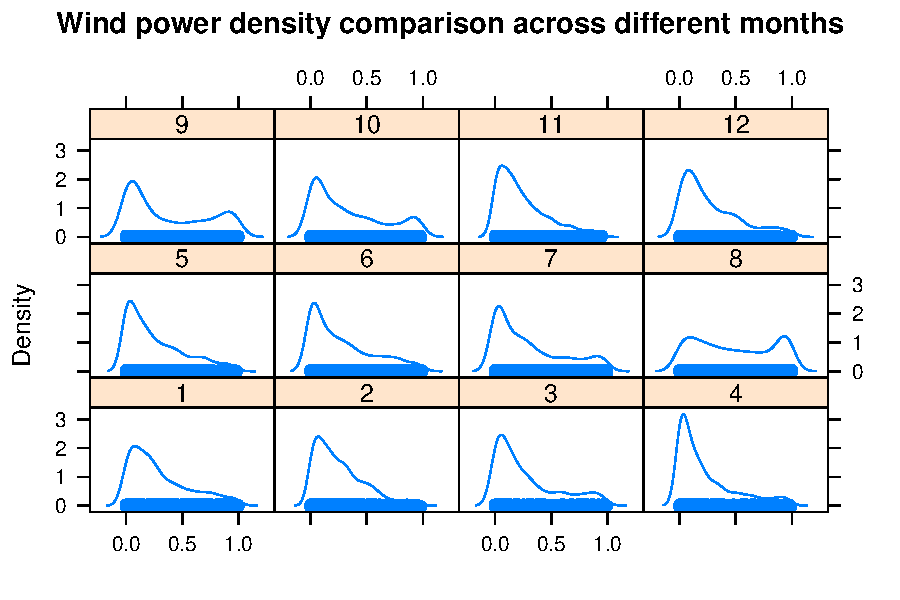
\includegraphics[width=0.9\linewidth]{Images/density}
\end{figure}

\end{frame}

\begin{frame}{The nongaussianity of Wind Power}

\begin{itemize}

\item
Renewables, such as wind and solar power have reportedly nongaussian
behaviour
\item
Convenience of using a nonparametric approach, which doesn't rely on
assuming a distribution
\item
Quantile regression is the chosen technique available to model this
time series dynamics, by estimating a thin grid of
\(\alpha\)-quantiles at once and forming a data-driven conditional
distribution
\end{itemize}

\end{frame}

\begin{frame}{Objectives}

\begin{itemize}
\item A nonparametric methodology to model the conditional distribution of renewables time series to produce scenarios.

\item We propose a methodology that selects the global optimal solution with parsimony both on the selection of covariates as on the quantiles. Regularization methods are based on two techniques: Best Subset Selection (MILP) and LASSO (Linear Programming) 

\item Regularization techniques applied to an ensemble of quantile functions to estimate the conditional distribution, solving the issue of non-crossing quantiles. On regularizing quantiles, we propose a smoothness on the coefficients values across the sequence of quantiles. 

\end{itemize}

\end{frame}

\section{Quantile Regression}\label{quantile-regression}

\begin{frame}{Definition of the Conditional Quantile}

Let the conditional quantile function of \(Y\) for a given value \(x\)
of the \(d\)-dimensional random variable \(X\), i.e.,
\(Q_{Y|X}:[0,1] \times \mathbb{R}^d \rightarrow \mathbb{R}\), can be
defined as:
\[Q_{Y|X}(\alpha,x) = F_{Y|X=x}^{-1}(\alpha) = \inf\{y: F_{Y|X=x}(y) \geq \alpha\}.\]

\end{frame}

\begin{frame}{Conditional Quantile from a sample}

Let a dataset be composed from \(\{y_t,x_t \}_{t \in T}\) and let
\(\rho\) be the check function

\begin{equation}\label{eq:check-function}
\rho_{\alpha}(x)=\begin{cases}
\alpha x & \text{if }x\geq0\\
(1-\alpha)x & \text{if }x<0
\end{cases},
\end{equation}

The sample quantile function for a given probability \(\alpha\) is then
based on a finite number of observations and is the solution to
minimizing the loss function \(L(\cdot)\): \[
\hat{Q}_{Y|X}(\alpha,\cdot)\quad\in\quad  \underset{q(\cdot)\in\mathcal{Q}}{\text{arg min}}\, L_\alpha(q) = \sum_{t\in T}\rho_{\alpha}(y_{t}-q(x_t)), 
\] \[
q(x_t) = \beta_0 + \beta^T x_t,
\] where \(\mathcal{Q}\) is a space of functions. In this paper, we use
\(\mathcal{Q}\) as an \textbf{affine functions space}.

\end{frame}

\begin{frame}{Conditional Quantile from a sample}

\begin{itemize}

\item
For a single quantile, this problem can be solved by the following
Linear Programming problem: \[
\begin{array}{lll}
\underset{\beta_0, \beta,\varepsilon_{t}^{+}, \varepsilon_{t}^{-}}{\text{min}} & \sum_{t \in T} \left(\alpha \varepsilon_{t}^{+}+(1-\alpha)\varepsilon_{t}^{-}\right) & \\
\mbox{s.t. } & \varepsilon_{t}^{+}-\varepsilon_{t}^{-}=y_{t} - \beta_{0} - \beta^T x_{t}, & \qquad\forall t \in T,\\
& \varepsilon_t^+,\varepsilon_t^- \geq 0, & \qquad \forall t \in T.
\end{array}
\]
\item
The output are the coefficients \(\beta_0\) and \(\beta\) (which is
the same dimension as \(x_t\)), that describe the quantile function as
an affine function.
\end{itemize}

\end{frame}

\begin{frame}{The non-crossing issue}

\begin{itemize}
	\item The following condition must always hold:
	$$q_\alpha(x_t) \leq q_{\alpha'}(x_t) \text{, when } \alpha \leq \alpha'$$
\end{itemize}

\begin{figure}
\centering
\begin{minipage}[t]{\linewidth}
\centering
\begin{minipage}[t]{0.45\linewidth}
\centering     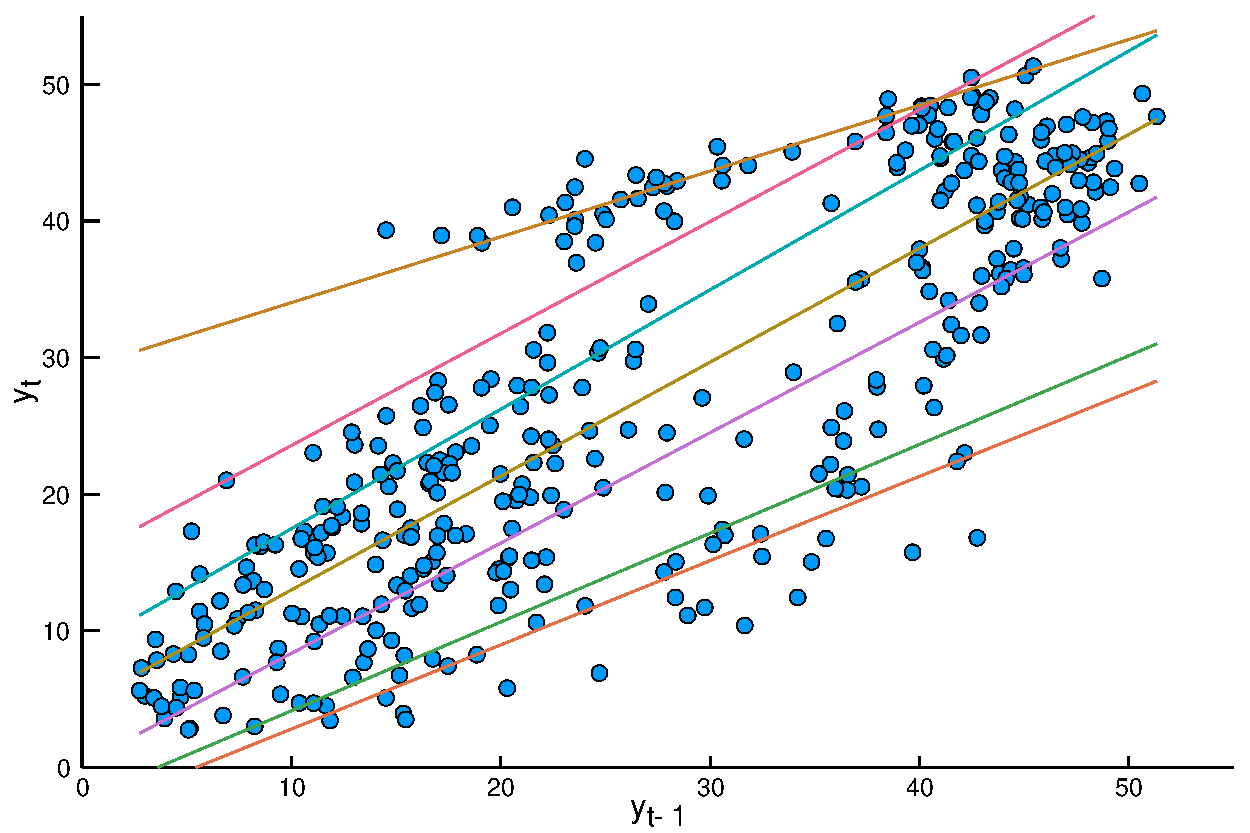
\includegraphics[width=\textwidth]{Images/icaraizinho-quantile-linear-scatter-crossing}
\subcaption{Each $\alpha$-quantile estimated independently}
\end{minipage}
\begin{minipage}[t]{0.45\linewidth}
\centering     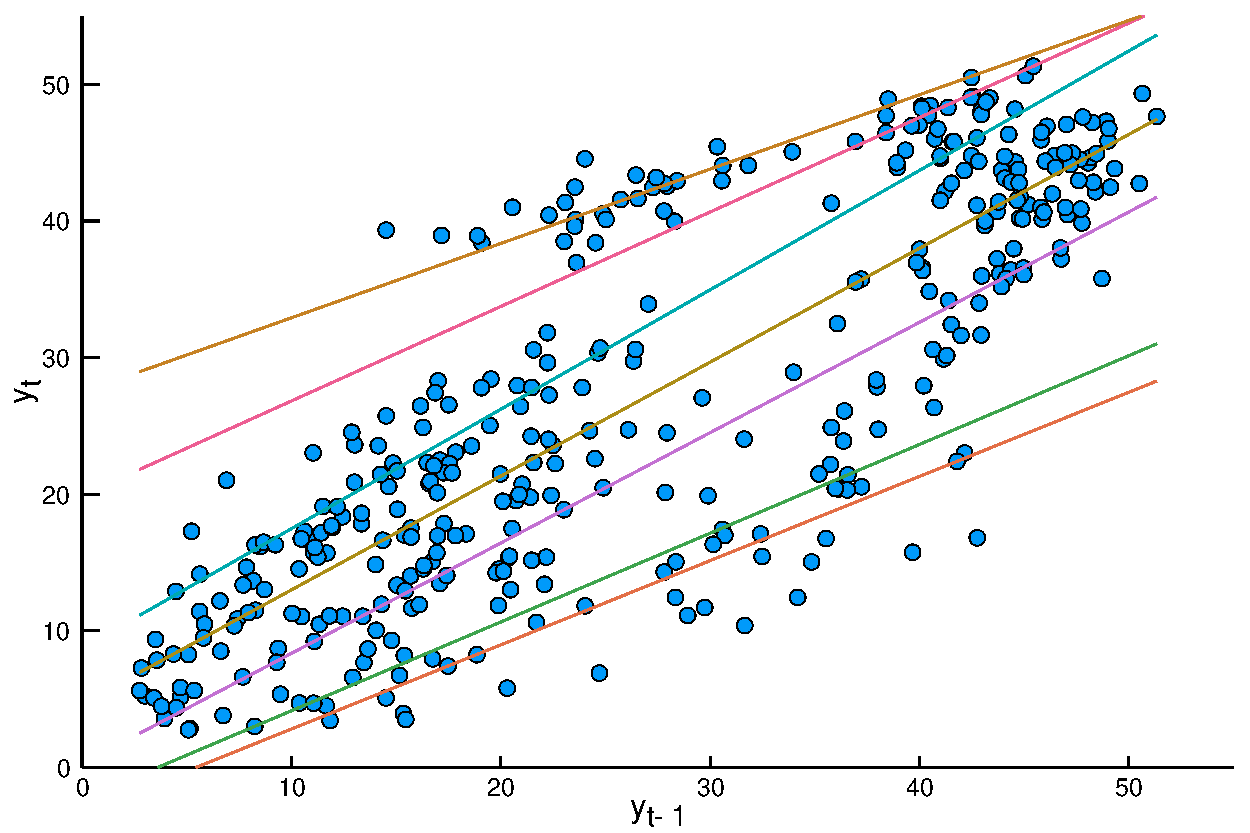
\includegraphics[width=\textwidth]{Images/icaraizinho-quantile-linear-scatter}
\subcaption{Estimation with non-crossing constraint}
\end{minipage}
\end{minipage}
\caption{These graphs show how the addition of a constraint can contour the crossing quantile issue}
\label{fig:quantiles-vs-xt}
\end{figure}

\end{frame}

\begin{frame}{Notation}

\small

\begin{longtable}[]{@{}ll@{}}
\toprule
\begin{minipage}[b]{0.14\columnwidth}\raggedright\strut
Expression\strut
\end{minipage} & \begin{minipage}[b]{0.80\columnwidth}\raggedright\strut
Meaning\strut
\end{minipage}\tabularnewline
\midrule
\endhead
\begin{minipage}[t]{0.14\columnwidth}\raggedright\strut
\(Q_{Y \mid X}(\alpha,x)\)\strut
\end{minipage} & \begin{minipage}[t]{0.80\columnwidth}\raggedright\strut
The conditional quantile function\strut
\end{minipage}\tabularnewline
\begin{minipage}[t]{0.14\columnwidth}\raggedright\strut
\(y_t\)\strut
\end{minipage} & \begin{minipage}[t]{0.80\columnwidth}\raggedright\strut
the time series we are modelling\strut
\end{minipage}\tabularnewline
\begin{minipage}[t]{0.14\columnwidth}\raggedright\strut
\(x_t\)\strut
\end{minipage} & \begin{minipage}[t]{0.80\columnwidth}\raggedright\strut
explanatory variables of \(y_t\) in \(t\)\strut
\end{minipage}\tabularnewline
\begin{minipage}[t]{0.14\columnwidth}\raggedright\strut
\(T\)\strut
\end{minipage} & \begin{minipage}[t]{0.80\columnwidth}\raggedright\strut
the set containing all observations indexes\strut
\end{minipage}\tabularnewline
\begin{minipage}[t]{0.14\columnwidth}\raggedright\strut
\(J\)\strut
\end{minipage} & \begin{minipage}[t]{0.80\columnwidth}\raggedright\strut
the set containing all quantile indexes\strut
\end{minipage}\tabularnewline
\begin{minipage}[t]{0.14\columnwidth}\raggedright\strut
\(J_{(-1)}\)\strut
\end{minipage} & \begin{minipage}[t]{0.80\columnwidth}\raggedright\strut
the set \(J\backslash \{1\}\)\strut
\end{minipage}\tabularnewline
\begin{minipage}[t]{0.14\columnwidth}\raggedright\strut
\(\alpha_j\)\strut
\end{minipage} & \begin{minipage}[t]{0.80\columnwidth}\raggedright\strut
a probability, might be indexed by \(j\)\strut
\end{minipage}\tabularnewline
\begin{minipage}[t]{0.14\columnwidth}\raggedright\strut
\(A\)\strut
\end{minipage} & \begin{minipage}[t]{0.80\columnwidth}\raggedright\strut
the set of probabilities \(\{\alpha_j \mid j \in J\}\)\strut
\end{minipage}\tabularnewline
\begin{minipage}[t]{0.14\columnwidth}\raggedright\strut
\(K\)\strut
\end{minipage} & \begin{minipage}[t]{0.80\columnwidth}\raggedright\strut
Maximum number of covariates on MILP regularization\strut
\end{minipage}\tabularnewline
\begin{minipage}[t]{0.14\columnwidth}\raggedright\strut
\(\lambda\)\strut
\end{minipage} & \begin{minipage}[t]{0.80\columnwidth}\raggedright\strut
The Lasso penalization on the coefficients \(\ell_1\)-norm\strut
\end{minipage}\tabularnewline
\begin{minipage}[t]{0.14\columnwidth}\raggedright\strut
\(\gamma\)\strut
\end{minipage} & \begin{minipage}[t]{0.80\columnwidth}\raggedright\strut
The penalization on the coefficients second-derivative with respect of
the quantiles\strut
\end{minipage}\tabularnewline
\bottomrule
\end{longtable}

\end{frame}

\begin{frame}{Conditional Quantile as a Linear Programming Problem}

\[
\min_{\beta_{0j},\beta_j,\varepsilon_{tj}^{+}, \varepsilon_{tj}^{-}} \, \sum_{j \in J} \sum_{t \in T}\left(\alpha_j \varepsilon_{t j}^{+}+(1-\alpha_j)\varepsilon_{t j}^{-}\right)
\] \[
\begin{array}{lr}
\text{s.t.} &\\
\varepsilon_{t j}^{+}-\varepsilon_{t j}^{-}=y_{t} - \beta_{0j} - \beta_{j}^T x_{t}, & \forall t \in T, \forall j \in J, \\
\varepsilon_{tj}^+,\varepsilon_{tj}^- \geq 0, & \forall t \in T,\forall j \in J,\\
\beta_{0,j-1} + \beta_{j-1}^T x_{t} \leq \beta_{0j} + \beta_{j}^T x_{t},
& \forall t \in T, \forall j \in J_{(-1)},
\end{array}
\]

\begin{itemize}
\item
Coefficients \(\beta_{0j}\) and \(\beta_j\) refer to the
\(j\)\textsuperscript{th} quantile
\item
We apply QR to estimate the conditional distribution
\(\hat{Q}_{Y_{t+h}|X_{t+h},Y_t, Y_{t-1}, \dots} (\alpha,\cdot)\) for a
\(k\)-step ahead forecast of time serie \(\{y_t\}\), where \(X_{t+h}\)
is a vector of exogenous variables at the time we want to forecast.
\end{itemize}

\end{frame}

\section{Regularization of
covariates}\label{regularization-of-covariates}

\begin{frame}{Best Subset selection via MILP}

\begin{itemize}

\item
Mixed Integer Linear Programming (MILP) models allow only \(K\)
variables to be used for each \(\alpha\)-quantile.
\item
Only \(K\) coefficients \(\beta_{pj}\) may have nonzero values, for
each \(\alpha\)-quantile.
\item
It is guaranteed by constraints on the optimization model.
\item
One model for each \(\alpha\)-quantile
\end{itemize}

\end{frame}

\begin{frame}{Best Subset selection via MILP}


\begin{IEEEeqnarray*}{llr}
\underset{\beta_{0j},\beta_j,z_{p j}, \varepsilon_{t j}^{+},\varepsilon_{t j}^{-}}{\text{min}} & \sum_{j \in J} \sum_{t\in T}\left(\alpha_j\varepsilon_{t j}^{+}+(1-\alpha_j)\varepsilon_{t j}^{-}\right)  & \\
\mbox{s.t } & \varepsilon_{t j}^{+}-\varepsilon_{t j}^{-}=y_{t}-\beta_{0 j}-\beta_{j}^T x_{t},& \forall t \in T ,\forall j \in J, \\
& \varepsilon_{t j}^{+},\varepsilon_{t j}^{-}\geq0,&\forall t \in T ,\forall j \in J, \\
& - M z_{p j} \leq \beta_{p j} \leq M z_{p j},& \forall j \in J, \forall p\in P, \\
& \sum_{p \in P} z_{p j} \leq K, &  \forall j \in J, \\
& z_{p j} \in \{0,1\},& \forall j \in J, \forall p\in P,\\
& \beta_{0,j-1} + \beta_{j-1}^T x_{t} \leq \beta_{0j} + \beta_{j}^T x_{t}, & \quad \forall t \in T, \forall j \in J_{(-1)},
\end{IEEEeqnarray*}


\begin{itemize}

\item
\(z_{pj}\) is a binary variable which indicates when
\(\beta_{pj} > 0\).
\end{itemize}

\end{frame}

\begin{frame}{Variable Selection via LASSO}

\begin{itemize}

\item
Regularization by including the coefficients \(\ell_1\)-norm on the
objective function.
\item
In this method, coefficients are shrunk towards zero by changing a
continuous parameter \(\lambda\), which penalizes the size of the
\(\ell_1\)-norm.\\
\item
When the value of \(\lambda\) gets bigger, fewer variables are
selected to be used.
\item
The optimization problem for a single quantile is presented below: 
\[
\underset{\beta_{0},\beta}{\text{min}} \sum_{t\in T}\rho_{\alpha}(y_{t}-(\beta_0 + \beta^T x_t))+\lambda\|\beta\|_{1},
\]
\end{itemize}

\end{frame}

\begin{frame}{Variable Selection via LASSO}

\begin{itemize}

\item
At first, we select variables using LASSO
\end{itemize}

\begin{IEEEeqnarray*}{lr}
\underset{\beta_{0},\beta,\varepsilon_{t j}^{+},\varepsilon_{t j}^{-}}{\text{arg min}} \sum_{j \in J} \sum_{t \in T}\left(\alpha_j \varepsilon_{t j}^{+}+(1-\alpha_j)\varepsilon_{t j}^{-}\right)+\lambda\sum_{p \in P}\mbox{\ensuremath{\xi}}_{p j} \span \label{eq:obj-lasso} \\
\mbox{subject to} \span \\
\varepsilon_{t j}^{+}-\varepsilon_{t j}^{-}= y_{t}-\beta_{0 j}-\beta_{j}^T x_{t},&\forall t\in T, \forall j \in J, \\
\varepsilon_{t j}^{+},\varepsilon_{t j}^{-}\geq0,&\forall t \in T, \forall j \in J,\\
\xi_{p\alpha}\geq\beta_{p j},&\forall p\in P, \forall j \in J, 
\\
\xi_{p\alpha}\geq-\beta_{p j},&\forall p\in P, \forall j \in J\\
\beta_{0,j-1} + \beta_{j-1}^T x_{t} \leq \beta_{0j} + \beta_{j}^T x_{t}, & \quad \forall t \in T, \forall j \in J_{(-1)},\\
\end{IEEEeqnarray*}

\end{frame}

\begin{frame}{Variable Selection via LASSO}

\begin{itemize}
\item
We then define \(S_\lambda\) as the set of indexes of selected
variables given by \[
S_{\lambda} = \{ p \in \{ 1,\dots,P \} | \; |\beta^{*LASSO}_{\lambda,p}| \neq 0  \}.
\] Hence, we have that, for each \(p \in \{ 1,\dots,P \}\),
\[\beta^{*LASSO}_{\theta,p} = 0 \Longrightarrow \beta^{*}_{\theta,p} = 0.\]
\item
On the second stage, we estimate coefficients using a regular QR where
input variables are only the ones which belonging to \(S_\lambda\)
\end{itemize}

\end{frame}

\section{Regularization on the
quantiles}\label{regularization-on-the-quantiles}

\begin{frame}{MILP - Defining groups for \(\alpha\)-quantiles}


\begin{IEEEeqnarray*}{lll}
\underset{\beta_{0j},\beta_j,z_{p j}, \varepsilon_{t j}^{+},\varepsilon_{t j}^{-}}{\text{min}} & \sum_{j \in J} \sum_{t\in T}\left(\alpha_j\varepsilon_{t j}^{+}+(1-\alpha_j)\varepsilon_{t j}^{-}\right)  & \\
\mbox{s.t } & \varepsilon_{t j}^{+}-\varepsilon_{t j}^{-}=y_{t}-\beta_{0 j}-\beta_{j}^T x_{t},& \forall t \in T ,\forall j \in J, \\
& \varepsilon_{t j}^{+},\varepsilon_{t j}^{-}\geq0,&\forall t \in T ,\forall j \in 
J, \\
&\mathcal{Z}_{p j g} := 2 - ( 1-z_{pg}) - I_{gj}, & \\
& - M \mathcal{Z}_{p j g} \leq \beta_{p j} \leq M \mathcal{Z}_{p j g},& \forall j \in J, \forall p\in P, \forall g \in G   \\
& \sum_{p \in P} z_{p g} \leq K, &  \forall j \in J, \\
& \beta_{0,j-1} + \beta_{j-1}^T x_{t} \leq \beta_{0j} + \beta_{j}^T x_{t}, & \forall t \in T, \forall j \in J_{(-1)},\\
& I_{gj}, z_{pg} \in \{0,1\},& \forall p \in P,\forall g \in G, \\
& z_{p g} \in \{0,1\},& \forall j \in J, \forall p\in P,\\
\end{IEEEeqnarray*}


\end{frame}

\begin{frame}{MILP - Penalization of derivative}

\small

\begin{IEEEeqnarray*}{llr}
\underset{\beta_{0j},\beta_j,z_{p j} \varepsilon_{t j}^{+},\varepsilon_{t j}^{-}}{\text{min}} & \sum_{j \in J} \sum_{t\in T}\left(\alpha_j \varepsilon_{tj}^{+}+(1-\alpha_j)\varepsilon_{t\alpha}^{-}\right) + \gamma \sum_{j \in J'} D2_{pj} \span \\
\mbox{s.t } & \varepsilon_{t j}^{+}-\varepsilon_{t j}^{-}=y_{t}-\beta_{0 j}-\beta_{j}^T x_{t},& \forall t \in T ,\forall j \in J, \\
& \varepsilon_{t j}^{+},\varepsilon_{t j}^{-}\geq 0,&\forall t \in T ,\forall j \in J, \label{eq:mip2}\\
& - M z_{p j} \leq \beta_{p j} \leq M z_{p j},& \forall j \in J, \forall p\in P, \label{eq:mip3}\\
& \sum_{p \in P} z_{p j} \leq K, & \qquad \forall j \in J, \label{eq:mip4}\\
& z_{p j} \in \{0,1\},& \forall j \in J, \forall p\in P, \label{eq:mip5}\\
& \tilde{D}_{pj}^{2}:=\frac{\left(\frac{\beta_{p,j+1}-\beta_{pj}}{\alpha_{j+1}-\alpha_{j}}\right)-\left(\frac{\beta_{p,j}-\beta_{p,j-1}}{\alpha_{J}-\alpha_{j-1}}\right)}{\alpha_{j+1}-2\alpha_{j}+\alpha_{j-1}} \span\\
& D2_{pj} \geq  \tilde D_{pj}^{2} &  \forall j \in J_{(-1)}, \forall p\in P, \\
& D2_{pj} \geq  - \tilde D_{pj}^{2} &  \forall j \in J_{(-1)}, \forall p\in P,\\
& \beta_{0,j-1} + \beta_{j-1}^T x_{t} \leq \beta_{0j} + \beta_{j}^T x_{t}, & \quad \forall t \in T, \forall j \in J_{(-1)},
\end{IEEEeqnarray*}

\end{frame}

\begin{frame}{LASSO - Penalization of derivative}

\small

\begin{IEEEeqnarray*}{llr}
	\underset{\beta_{0},\beta,\varepsilon_{t j}^{+},\varepsilon_{t j}^{-}}{\text{min}} \sum_{j \in J} \sum_{t \in T}(\alpha_j\varepsilon_{t j}^{+}+(1-\alpha_j)\varepsilon_{t j}^{-}) +\lambda\sum_{p \in P}\mbox{\ensuremath{\xi}}_{p j} + \gamma \sum_{j \in J'} D2_{pj} \span \span \nonumber \\
	\mbox{s.t.} \qquad \ & \varepsilon_{t j}^{+}-\varepsilon_{t j}^{-}=y_{t}-\beta_{0 j}-\beta_{j}^T x_{t,p},& \forall t \in T ,\forall j \in J,\\
	& \varepsilon_{t j}^{+},\varepsilon_{t j}^{-}\geq0,&\forall t \in T, \forall j \in J,\\
	& \xi_{pj}\geq\beta_{p j},&\forall p\in P, \forall j \in J,  \label{l1-qar-3}
	\\
	& \xi_{pj}\geq - \beta_{p j},&\forall p\in P, \forall j \in J,  \label{l1-qar-4}
	\\
& \tilde{D}_{pj}^{2} := \frac{\left(\frac{\beta_{p,j+1}-\beta_{pj}}{\alpha_{j+1}-\alpha_{j}}\right)-\left(\frac{\beta_{p,j}-\beta_{p,j-1}}{\alpha_{j}-\alpha_{j-1}}\right)}{\alpha_{j+1}-2\alpha_{j}+\alpha_{j-1}}\\
& D2_{pj} \geq  \tilde D_{pj}^{2} &  \forall j \in J_{(-1)}, \forall p\in P, \\
& D2_{pj} \geq - \tilde D_{pj}^{2} &  \forall j \in J_{(-1)}, \forall p\in P,\\
& \beta_{0j} + \beta_{j}^T x_{t} \leq \beta_{0,j+1} + \beta_{j+1}^T x_{t},&\forall t \in T, \forall j \in J_{(-1)}, \label{eq:l1-qar5}
\end{IEEEeqnarray*}


%
%\begin{eqnarray*}
%\underset{\beta_{0},\beta,\varepsilon_{t j}^{+},\varepsilon_{t j}^{-}}{\text{arg min}} & \sum_{j \in J} \sum_{t \in T}\left(\alpha_j \varepsilon_{t j}^{+}+(1-\alpha_j)\varepsilon_{t j}^{-}\right)+\lambda\sum_{p=1}^{P}\mbox{\ensuremath{\xi}}_{p j} + \gamma \sum_{j \in J'} D2_{pj} \span \label{eq:obj-lasso} \\
%\mbox{s.t. } & \varepsilon_{t j}^{+}-\varepsilon_{t j}^{-}= y_{t}-\beta_{0 j}-\sum_{p=1}^{P}\beta_{p j}\tilde x_{t,p},&\forall t\in T, \forall j \in J, \\
%& \varepsilon_{t j}^{+},\varepsilon_{t j}^{-}\geq0,&\forall t \in T, \forall j \in J,\\
%& \xi_{p\alpha}\geq\beta_{p j},&\forall p\in P, \forall j \in J,  \label{l1-qar-3}
%\\
%& \tilde{D}_{pj}^{2}=\frac{\left(\frac{\beta_{p,j+1}-\beta_{pj}}{\alpha_{j+1}-\alpha_{j}}\right)-\left(\frac{\beta_{p,j}-\beta_{p,j-1}}{\alpha_{J}-\alpha_{j-1}}\right)}{\alpha_{j+1}-2\alpha_{j}+\alpha_{j-1}} \span\\
%& D2_{pj} >  \tilde D_{pj}^{2} &  \forall j \in J_{(-1)}, \forall p\in P, \\
%& D2_{pj} >  - \tilde D_{pj}^{2} &  \forall j \in J_{(-1)}, \forall p\in P,\\
%& \beta_{0,j-1} + \beta_{j-1}^T x_{t} \leq \beta_{0j} + \beta_{j}^T x_{t}, & \forall t \in T, \forall j \in J_{(-1)},\\
%& \xi_{pj}\geq-\beta_{p j},&\forall p\in P, \forall j \in J. 
%\end{eqnarray*}

\end{frame}

\begin{frame}{LASSO - Penalization of derivative}

\begin{figure}
\centering
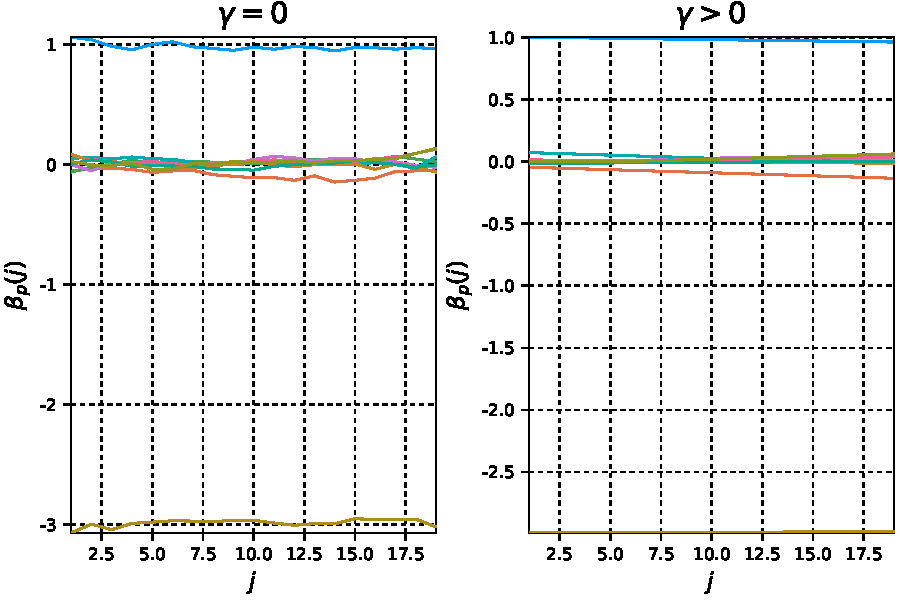
\includegraphics[width=0.9\linewidth]{Images/Lambda10-gamma03.pdf}
\end{figure}

\end{frame}

\begin{frame}{LASSO - Penalization of derivative}

\begin{figure}
\centering
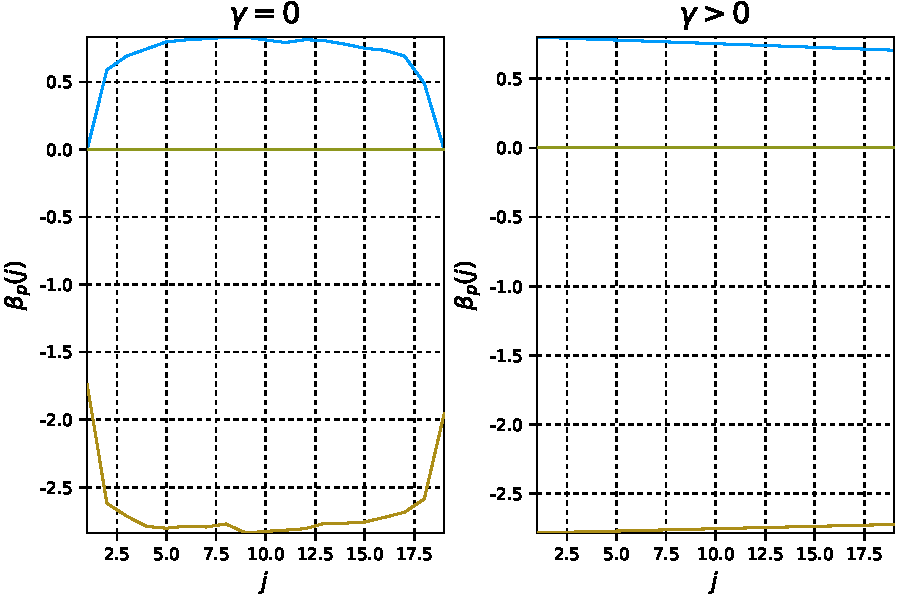
\includegraphics[width=0.9\linewidth]{Images/Lambda500-gamma30.pdf}
\end{figure}

\end{frame}

\begin{frame}{LASSO - Penalization of derivative}

\begin{figure}
\centering
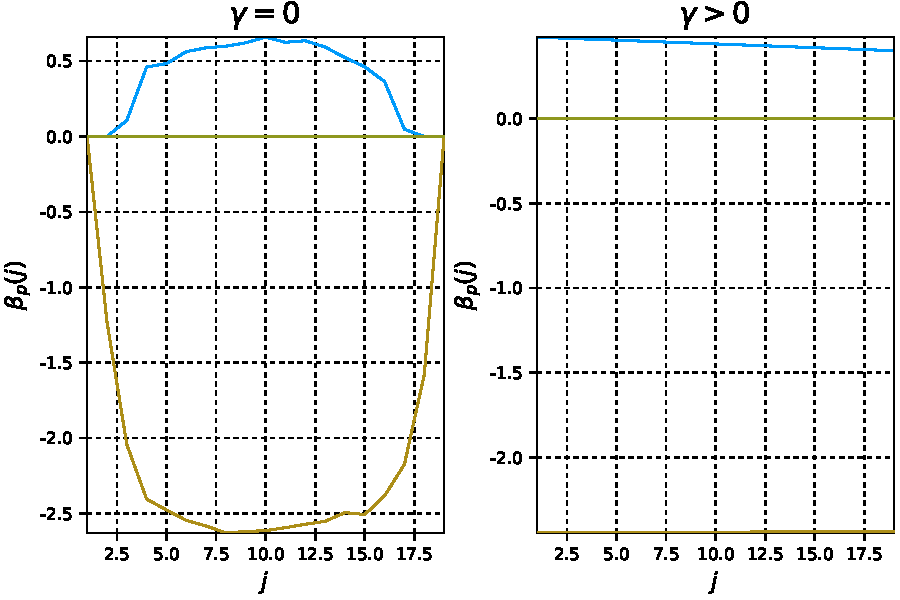
\includegraphics[width=0.7\linewidth]{Images/Lambda1000-gamma100.pdf}
\caption{Testing caption}
\end{figure}

\end{frame}


\begin{frame}{ADALASSO}

\small
LASSO solutions are solutions that minimize

\[
Q(\beta|X,y)=\frac{1}{2n}\parallel y-X\beta\parallel^{2}+\lambda\sum_{p \in P}\mid\beta_{p}\mid.
\]
The adaptive lasso simply adds weights to this to try to counteract
the known issue of LASSO estimates being biased. 

\[
Q_{a}(\beta|X,y,w)=\frac{1}{2n}\parallel y-X\beta\parallel^{2}+\lambda\sum_{p \in P}w_{p}\mid\beta_{p}\mid.
\]
Often you will see $w_p=1/\tilde{\beta}_{p}$, where $\tilde{\beta}_{p}$
are some initial estimates of the $\beta$ (maybe from just using
LASSO, or using least squares, etc). Sometimes adaptive lasso is fit
using a pathwise approach where the
weight is allowed to change with $\lambda$:

\[
w_{p}(\lambda)=w(\tilde{\beta}_{p,t}(\lambda)).
\]
In the \textbf{glmnet} package the weights can be specified with the
penalty.factor argument. I'm not sure if you can specify the pathwise
approach in glmnet.

\end{frame}


\begin{frame}{ADALASSO for quantiles}
	

\small
The problem modified for quantiles

\begin{itemize}
	\item \textbf{First step:} Normal lasso regularization
	\[
\underset{\beta_{0j},\beta_j}{\text{min}} \sum_{j \in J} \left( \sum_{t\in T}\rho_{\alpha_j}(y_{t}-(\beta_{0j} + \beta_j^T x_t)) + \lambda\  \sum_{p \in P} \mid  \beta_{pj} \mid \right),
\]
	

	
	\item \textbf{Second step:} Use initial estimation to determine $w_{pj}$. We can use two different approaches:
	\begin{enumerate}
		\item $w_{pj} = 1/ \parallel \beta_j \parallel_1$,
		\item $w_{pj} = 1/ \beta_{pj}$.
	\end{enumerate}
	The weights $w_j$ are input to a second-stage Lasso estimation:
		\[
	\underset{\beta_{0j},\beta_j}{\text{min}} \sum_{j \in J} \left( \sum_{t\in T}\rho_{\alpha_j}(y_{t}-(\beta_{0j} + \beta_j^T x_t)) + \lambda\  \sum_{p \in P} w_{pj}^\delta \mid  \beta_{pj} \mid \right),
	\]
	where $\delta$ is an exponential parameter, normally set to 1.
	
\end{itemize}



\end{frame}

\section{Estimation and Evaluation}\label{estimation-and-evaluation}

\begin{frame}{Evaluation Metrics}

\begin{itemize}

\item
We use a performance measurement which emphasizes the correctness of
each quantile. For each probability \(\alpha \in A\), a loss function
is defined by
\[L_\alpha(q)= \sum_{t\in T}\rho_{\alpha}(y_{t}-q_{\alpha}(x_t)).\]
The loss score \(\mathcal{L}\), which is the chosen evaluation metric
to optimize, aggregates the score function over all elements of \(A\):
\[\mathcal{L}= \frac{1}{|A|}\sum_{\alpha \in A}L_\alpha(q).\]
\end{itemize}

\end{frame}

\begin{frame}{Time-series Cross-Validation}

\begin{figure}
\centering
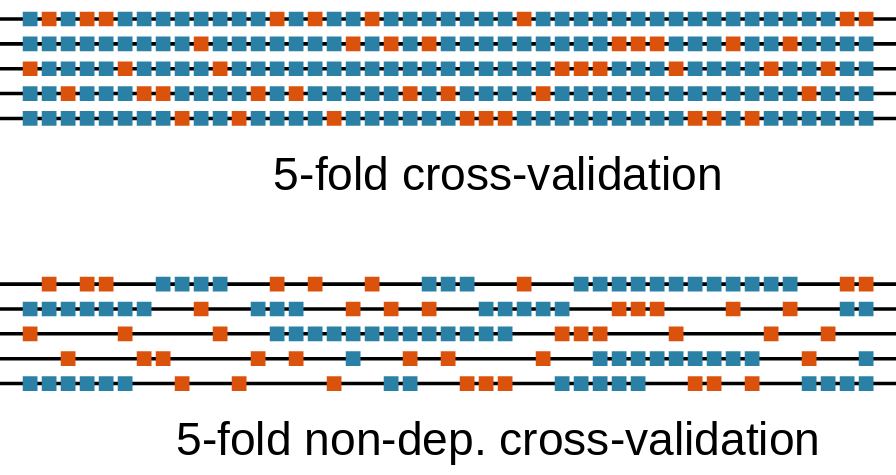
\includegraphics[width=0.9\linewidth]{Images/Cross-validation-scheme}
\caption{$\mathcal{K}$-fold CV and $\mathcal{K}$-fold with non-dependent data. Observations in blue are used to estimation and in orange for evaluation. Note that non-dependent data doesn't use all dataset in each fold.}
\label{fig:cross-validation-scheme}
\end{figure}

\end{frame}

\begin{frame}{Time-series Cross-Validation}

\begin{itemize}

\item
The CV score is given by the sum of the loss function for each fold.
The optimum value of \(t\) in this criteria is the one that minimizes
the CV score: \[
\theta^* = \text{argmin}_\theta CV(\theta) = \sum_{k \in \mathcal{K}} \sum_{\alpha \in A} L_\alpha(q).
\]
\item
To optimize CV function in \(\theta\), we use the Nelder-Mead
algorithm, which is a known and widely used algorithm for black-box
optimization.
\end{itemize}

\end{frame}

\section{Nonparametric model}\label{nonparametric-model}

\begin{frame}{Nonparametric model}

\[
\hat{Q}_{Y|X}(\alpha,\cdot)\quad\in\quad  \underset{q(\cdot)\in\mathcal{Q}}{\text{arg min}}\, L_\alpha(q) = \sum_{t\in T}\rho_{\alpha}(y_{t}-q(x_t)),
\]

\begin{itemize}
\item
On nonparametric models, \(q_\alpha\) belongs to a space of limited
second derivative function \(\mathcal{Q}\).
\item
The \(\alpha\)-quantile function is flexible enough to capture
nonlinearities on the quantile function.
\end{itemize}

\end{frame}

\begin{frame}{Nonparametric model - Formulation}


\begin{IEEEeqnarray*}{llr}
\min_{q_{j t},\varepsilon^+_{t}, \varepsilon_t^-, \xi_t} \sum_{j \in J} \sum_{t \in T'}\left(\alpha_j \varepsilon_{t j }^{+}+(1-\alpha_j)\varepsilon_{t j }^{-}\right) + \lambda \sum_{t \in T'}\xi_{t j } \span \span \nonumber \\
s.t. \qquad & \varepsilon_{t}^{+}-\varepsilon_{t j }^{-}=y_{t}-q_{t j }, & \forall t \in T',\forall j \in J,\\
& D^{1}_{t j }=\frac{q_{j t+1}-q_{j t}}{x_{t+1}-x_{t}}, 
& \qquad\forall t \in T',\forall j \in J,\\   
& D^{2}_{t j }:=\frac{\left(\frac{q_{j t+1}-q_{j t}}{x_{t+1}-x_{t}}\right)-\left(\frac{q_{j t}-q_{j t-1}}{x_{t}-x_{t-1}}\right)}{x_{t+1}-2x_{t} + x_{t-1}} \span\\
& \xi_{t j}\geq D^2_{t j }, & \qquad\forall t \in T',\forall j \in J,\\
& \xi_{t j}\geq-D^2_{t j}, & \qquad\forall t \in T',\forall j \in J,\\
& \varepsilon_{t j}^{+},\varepsilon_{t j}^{-}, \xi_{t j}\geq0, & \qquad\forall t \in T',\forall j \in J,\\
& q_{t j} \leq q_{t,j+1}, & \qquad \forall t \in T', \forall j \in J,\nonumber \\  
\end{IEEEeqnarray*}


\end{frame}

\begin{frame}{Nonparametric vs.~Linear Model}

\begin{itemize}

\item
The nonparametric approach is more flexible to capture
heteroscedasticity.
\end{itemize}

\begin{figure}
\centering
\begin{minipage}[t]{\linewidth}
\centering
\begin{minipage}[t]{0.45\linewidth}
\centering     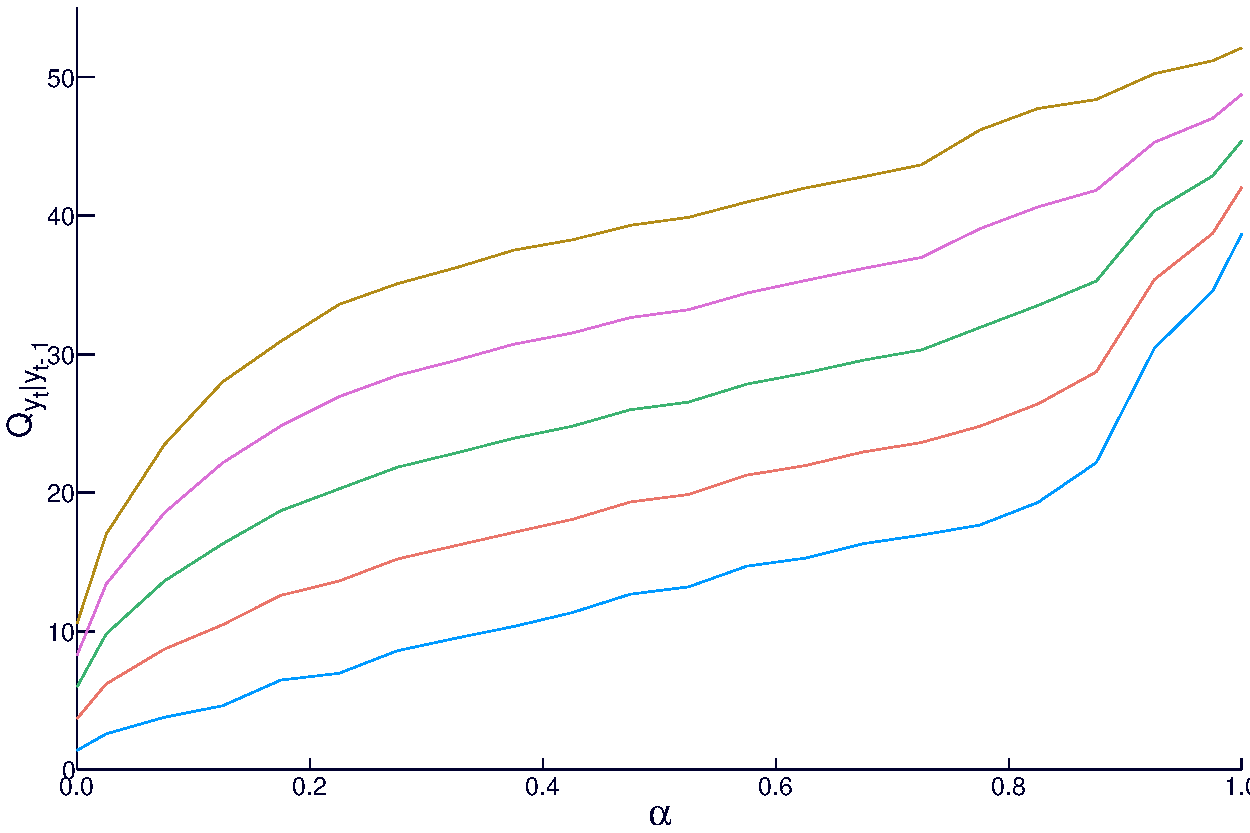
\includegraphics[width=\textwidth]{../Figuras/regressao-quantilica/icaraizinho-quantile-linear}
\end{minipage}
\begin{minipage}[t]{0.45\linewidth}
\centering     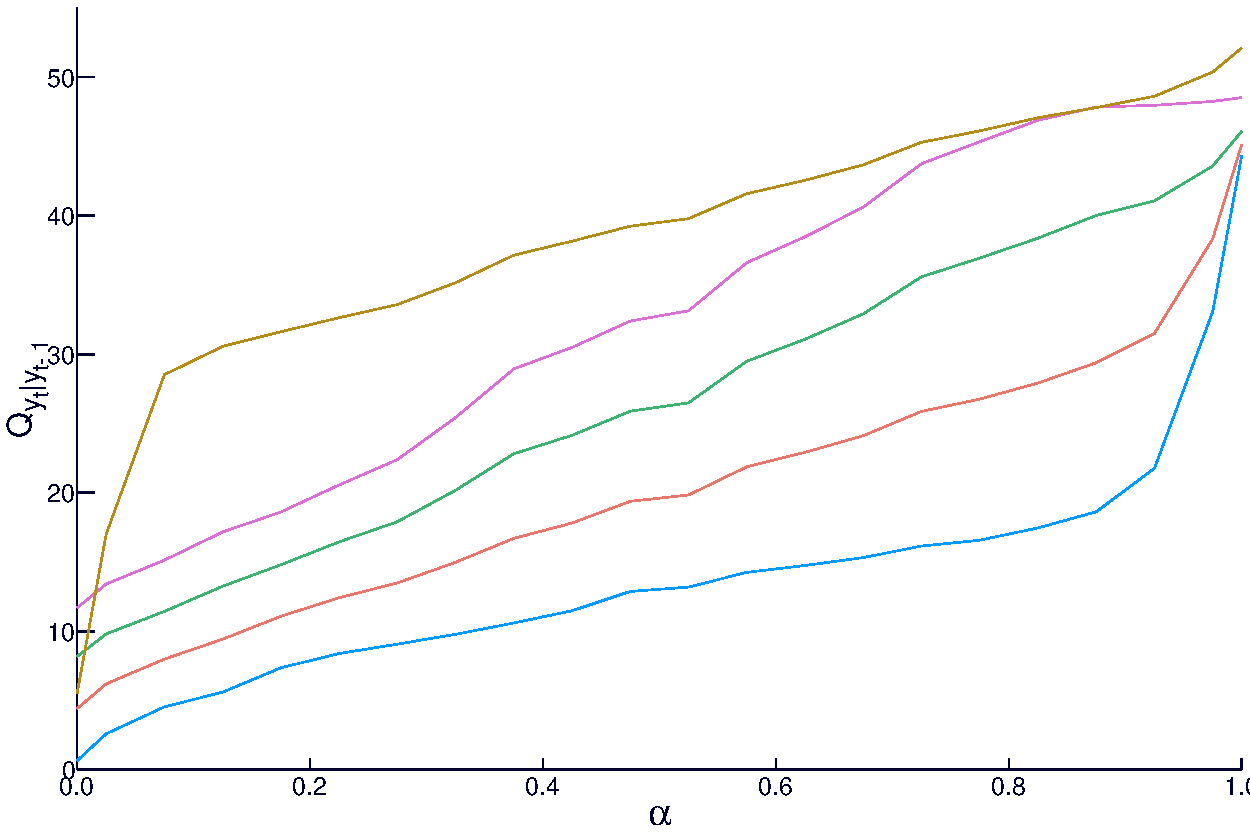
\includegraphics[width=\textwidth]{../Figuras/regressao-quantilica/icaraizinho-quantile-nonpar-lambda30}
\end{minipage}
\end{minipage}
\caption{Estimated quantile functions, for different values of $y_{t-1}$. On the left using a linear model and using a nonparametric approach on the right.}
\label{fig:quantiles-vs-xt}
\end{figure}

\end{frame}

\begin{frame}{Control of smoothing parameter}

\begin{itemize}

\item
This flexibility might lead to overfitting, if we don't select a
proper smoothing parameter.
\end{itemize}

\begin{figure}
\centering
\begin{minipage}[t]{\linewidth}
\centering
\begin{minipage}[t]{0.45\linewidth}
\centering     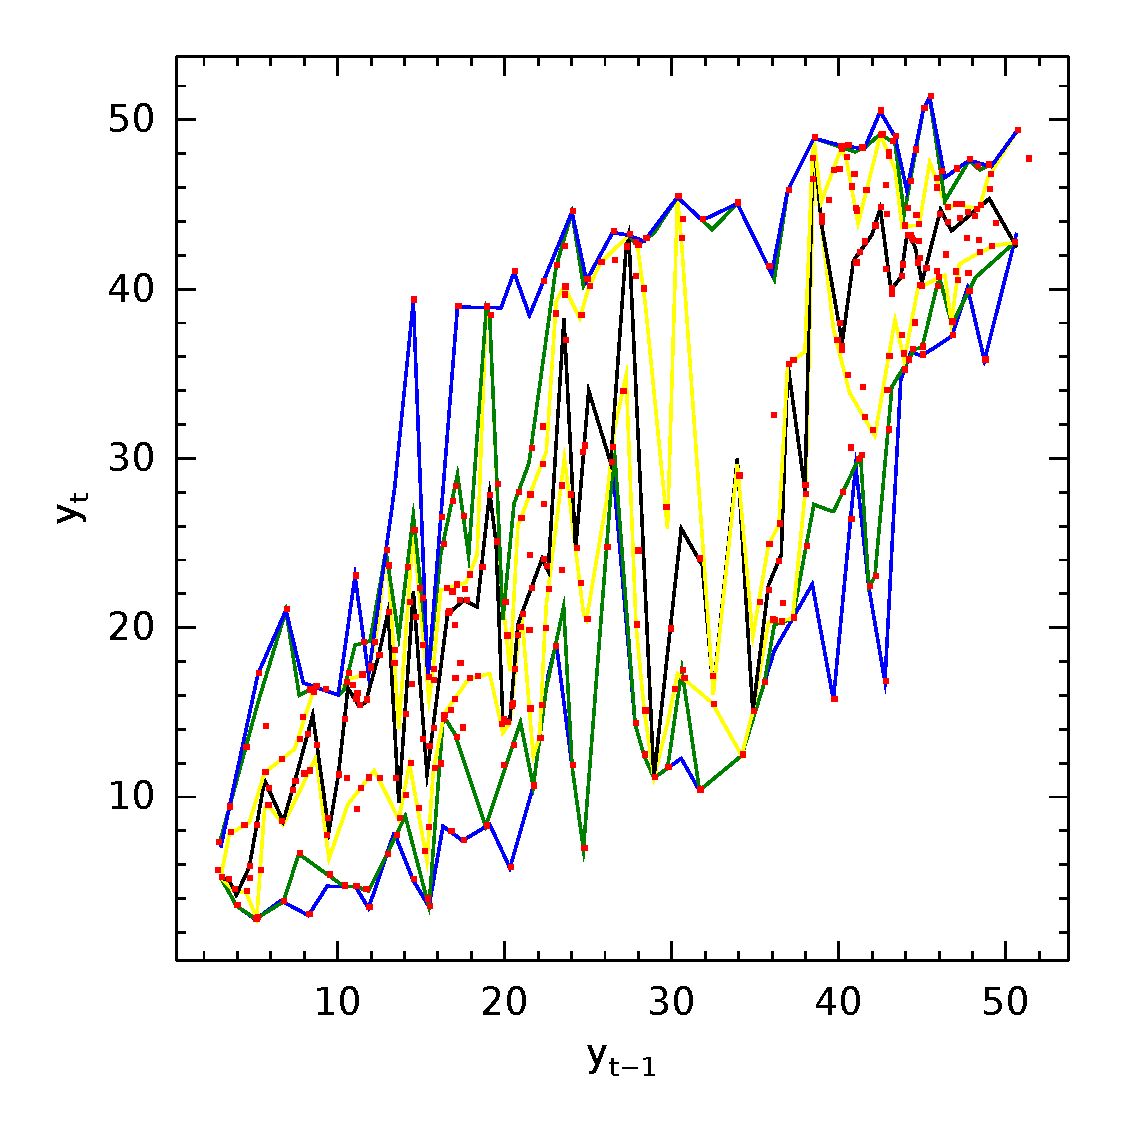
\includegraphics[width=\textwidth]{../Figuras/npqar/icaraizinho-crossing-01}
\subcaption{$\lambda = 0.1$}
\end{minipage}
\begin{minipage}[t]{0.45\linewidth}
\centering     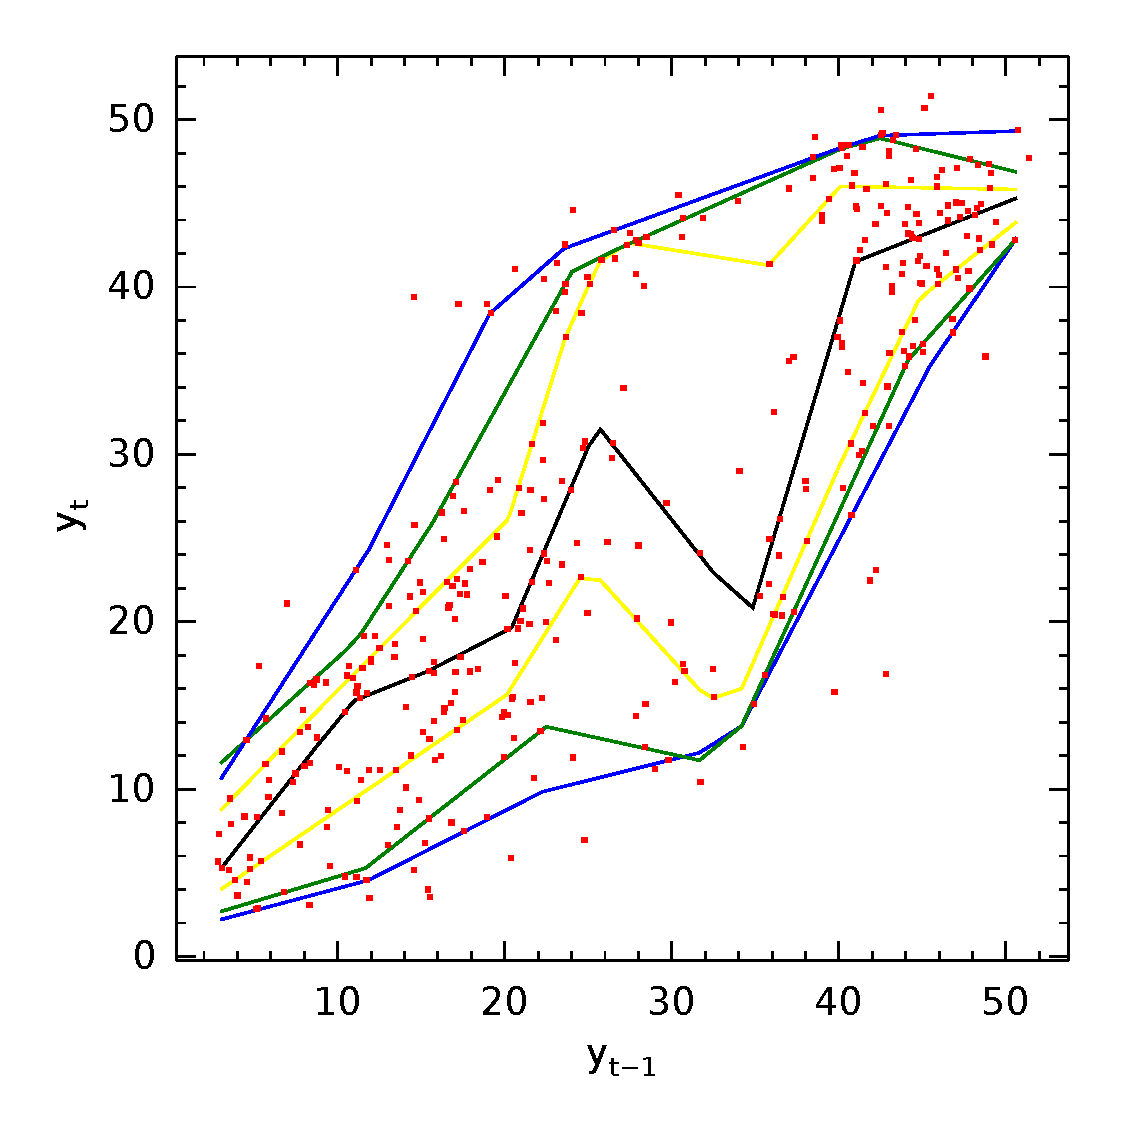
\includegraphics[width=\textwidth]{../Figuras/npqar/icaraizinho-crossing-3}
\subcaption{$\lambda = 3$}
\end{minipage}
\end{minipage}
\end{figure}

\end{frame}

\begin{frame}{Control of smoothing parameter}

\begin{figure}
\centering
\begin{minipage}[t]{\linewidth}
\centering
\begin{minipage}[t]{0.45\linewidth}
\centering     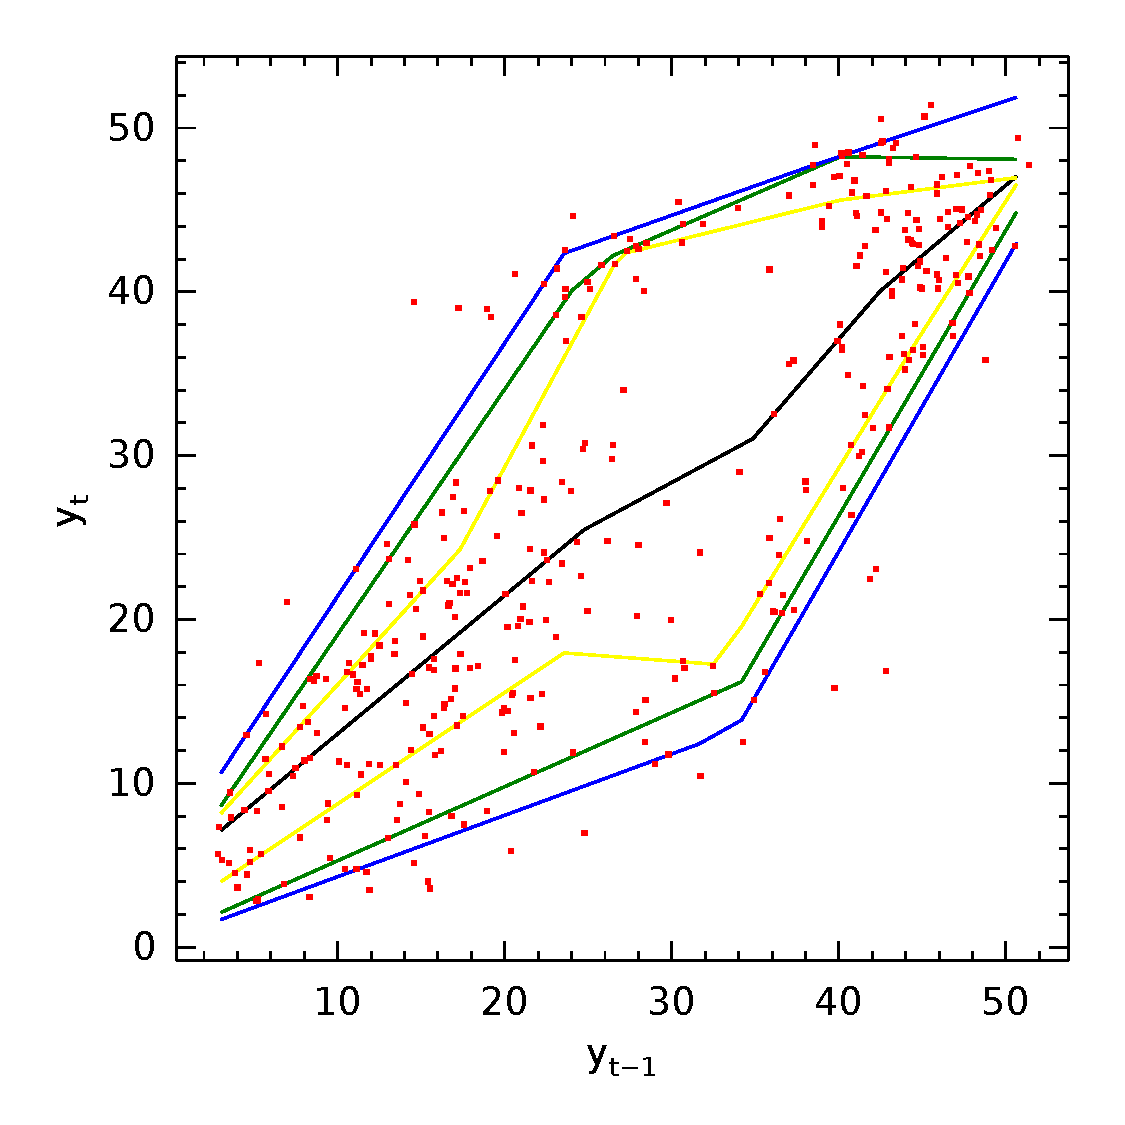
\includegraphics[width=\textwidth]{../Figuras/npqar/icaraizinho-crossing-10}
\subcaption{$\lambda = 10$}
\end{minipage}
\begin{minipage}[t]{0.45\linewidth}
\centering     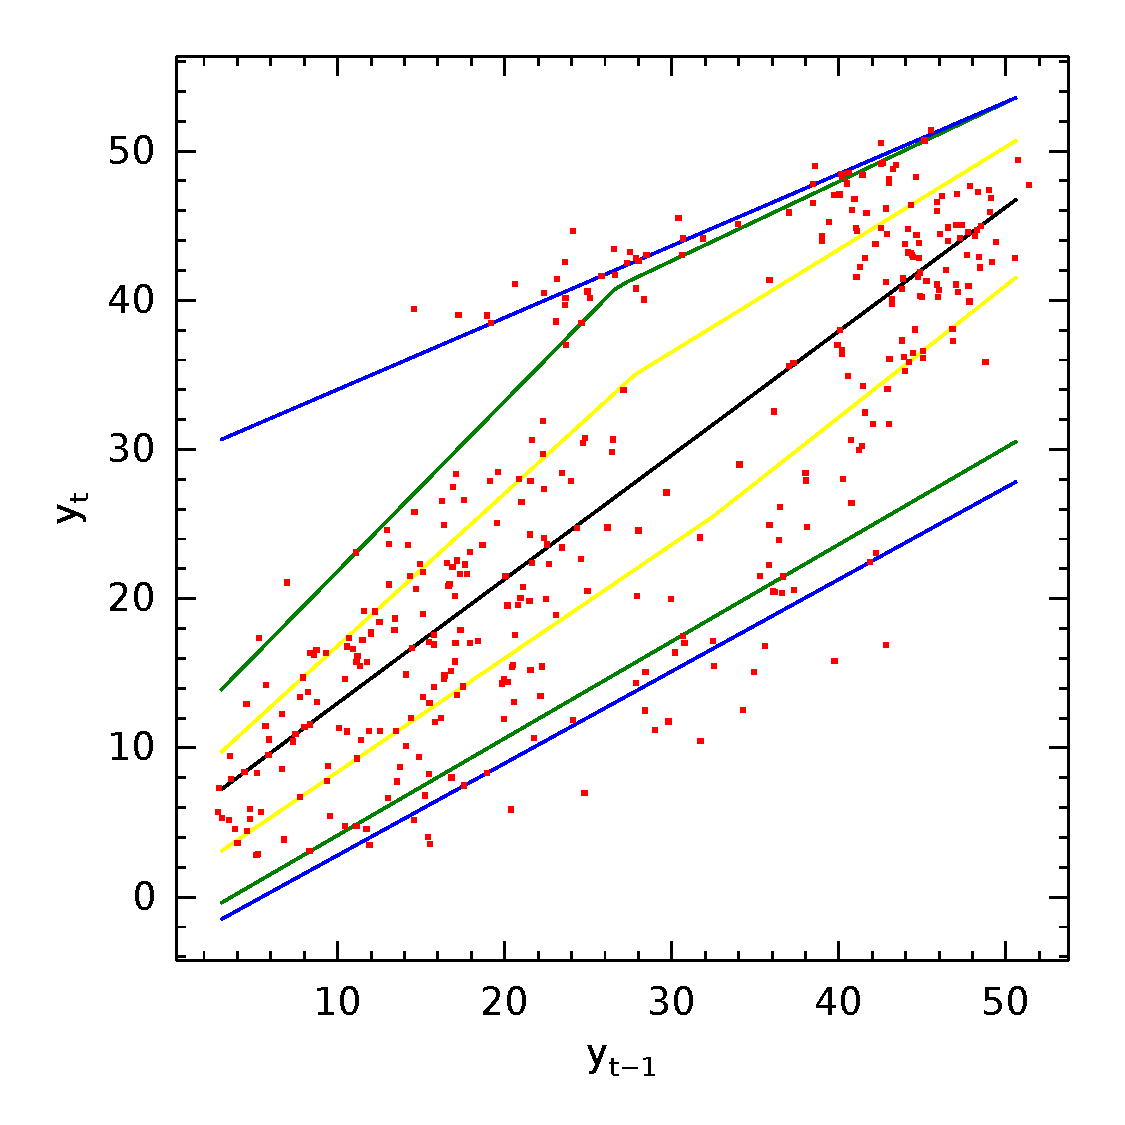
\includegraphics[width=\textwidth]{../Figuras/npqar/icaraizinho-crossing-100}
\subcaption{$\lambda = 100$}
\end{minipage}
\end{minipage}
\end{figure}

\begin{itemize}

\item
On the limit, when \(\lambda \rightarrow \infty\), the nonparametric
model approaches a linear model.
\end{itemize}

\end{frame}

\begin{frame}{Present issues}

\begin{itemize}

\item
Difficult interpolation when \(x_t\) has dimension greater than 1.
\item
Control of smoothing parameter
\end{itemize}

\end{frame}

\section{Final}\label{final}

\begin{frame}{References}

\tiny

\hypertarget{refs}{}
\hypertarget{ref-gallego2016line}{}
Gallego-Castillo, Cristobal, Ricardo Bessa, Laura Cavalcante, and Oscar
Lopez-Garcia. 2016. ``On-Line Quantile Regression in the Rkhs
(Reproducing Kernel Hilbert Space) for Operational Probabilistic
Forecasting of Wind Power.'' \emph{Energy} 113. Elsevier: 355--65.

\hypertarget{ref-koenker1978regression}{}
Koenker, Roger, and Gilbert Bassett Jr. 1978. ``Regression Quantiles.''
\emph{Econometrica: Journal of the Econometric Society}. JSTOR, 33--50.

\hypertarget{ref-wan_direct_2017}{}
Wan, C., J. Lin, J. Wang, Y. Song, and Z. Y. Dong. 2017. ``Direct
Quantile Regression for Nonparametric Probabilistic Forecasting of Wind
Power Generation.'' \emph{IEEE Transactions on Power Systems} 32 (4):
2767--78.
doi:\href{https://doi.org/10.1109/TPWRS.2016.2625101}{10.1109/TPWRS.2016.2625101}.

\end{frame}

\end{document}
